\documentclass{beamer}
\usecolortheme{wolverine}

% math stuff
\usepackage{amsmath}
\usepackage{amsthm}
\usepackage{amssymb}
\usepackage{xcolor}

\usepackage{float}
\usepackage{subcaption}

% to insert images
\usepackage{graphicx}

% to correctly insert stressed characters
\usepackage[T1]{fontenc}
\usepackage[utf8]{inputenc}

\usepackage{multirow}

% Bibliography
% \usepackage[style=alphabetic]{biblatex}
% \usepackage[nottoc]{tocbibind}
% \usepackage{bibentry}
% \setcounter{biburllcpenalty}{9000}
% \usepackage{nameref}

% to put links in table of contents
\usepackage{hyperref}
\hypersetup{colorlinks=false, %set true if you want colored links
    linktoc=all,     %set to all if you
}

% Add symbols
% \usepackage{textcomp}

% Add command for Real and Z sets
% \usepackage{dsfont}
% \newcommand{\Rset}{$\mathds{R}$}
% \newcommand{\Zset}{$\mathds{Z}$}

% Code highlighting
% \usepackage{minted}
% \usemintedstyle{perldoc}
% \setminted{
%     frame=single,
%     breaklines,
% }

% tikz figures
% \usepackage{tikz}
% \input{style.tikzstyle}
% \usetikzlibrary{positioning}

\begin{document}
\title{Thesis notes}
\date{23rd February}
\frame{\titlepage}

\begin{frame}[c]
    \frametitle{A bigger graph on r/politics (1)}
    \begin{figure}[htpb]
        \centering
        \includegraphics[width=0.8\linewidth]{img/graph-politics.pdf}
    \end{figure}
    
\end{frame}

\begin{frame}[c]
    \frametitle{A bigger graph on r/politics (2)}
    \begin{itemize}
        \item Built on 200 posts
        \item The graph has 15569 vertices and 28239 edges
        \item Fraction of negative edges: 0.5100276380128977
        \item Clustering coefficient: 0.0030298911181069264
        \item Average shortest path length: 10.56448348380506
    \end{itemize}
\end{frame}

\begin{frame}[c]
    \frametitle{Reconstructing topics: a summary}
    \begin{enumerate}
        \item From the user-user graph find communities
        \item Build user-content graph by multiplying chain of comments.
            I.e. If user A replies to content C positively and B replies
            negatively to A, link B to C with a negative edge
        \item Find position of content with respect to communities (topic) and minimal
            set of articles definying on which side of the debate a user is
    \end{enumerate}
    
\end{frame}

\begin{frame}[c]
    \frametitle{About Twitter annotations}
    Twitter provides different categories which are associated to tweets

    \begin{figure}[htpb]
        \centering
        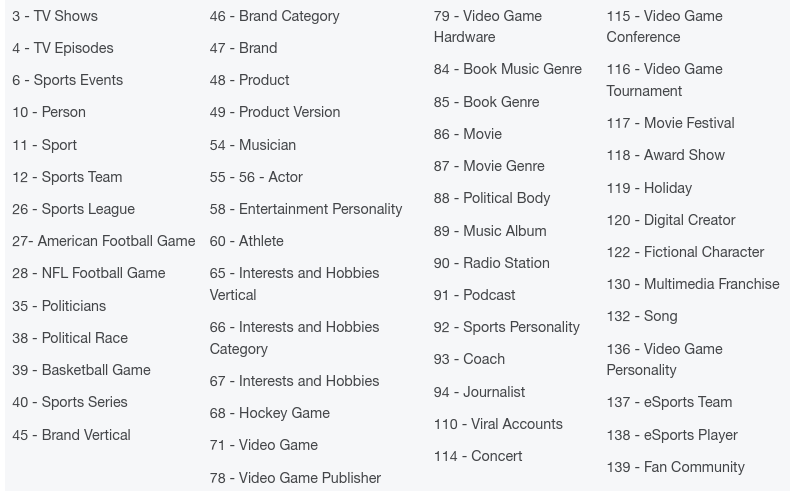
\includegraphics[width=0.8\linewidth]{img/twitter-categories.png}
    \end{figure}
\end{frame}

\begin{frame}[c]
    \frametitle{About Twitter annotations}
    But the results are not really satisfying

    \begin{figure}[htpb]
        \centering
        
\includegraphics[width=0.8\linewidth]{img/twitter-fauci.png}
    \end{figure}

    Annotations:
    \begin{itemize}
        \item Brand Vertical(Top level entities that describe a Brands industry):
            \textbf{Entertainment} , 
        \item Brand Category: (Categories within Brand Verticals that narrow down the
            scope of Brands): \textbf{Online Site},
        \item Brand Category (Categories within Brand Verticals that narrow
            down the scope of Brands): \textbf{TV/Movies Related},
        \item Brand(Brands and Companies): \textbf{Fox News},
        \item Interests and Hobbies Vertical(Top level interests and hobbies groupings,
            like Food or Travel): \textbf{Food}
        \item Interests and Hobbies Category(A grouping of interests and hobbies
            entities, like Novelty Food or Destinations): \textbf{Dining}
        \item Interests and Hobbies(Interests, opinions, and behaviors of individuals,
            groups, or cultures): \textbf{Dining out}
    \end{itemize}
\end{frame}

\end{document}


